\section{INTRODUCTION}
\label{sec:intro}

%I didn't like this intro :)
%The rising interest, research, and development of GPS devices have increased potential market significantly. With cheaper devices comes a larger number of potential applications.

%A constant feed of spatio-temporale points from the vehicle network, available in real-time with high accuracy, makes for an interesting market for a broader spectrum of companies.

GPS devices have grown to be incredibly popular over the last two decades, and are now used everywhere. Common examples include dedicated GPS navigators for cars and as integrated parts of smartphones.

With high interest and research into the technology, we now have high-frequency devices with good precision available at an affordable price point.\cite{art:telematicsmatter}

As a consequence of this development, markets are affected. Insurance companies are one of the markets where GPS technology has the potential to change the market. Car insurances has traditionally been based on the facts available at the time of purchase. Insurance companies will usually require detailed information about you and your car, creating an offer based on this. Coupled with historical statistics, an insurance company can make reasonable predictions about risks associated with insuring your car. For example, statistics often show young drivers being involved in more accidents compared to other age groups\cite{accidents}. This will usually result in a less attractive price for this group.

Basing insurance pricing on such wide prediction criteria is unfair for the individual customer. The generalization that young people are poor drivers means, that those who do drive well have to pay extra because of those who do not. The problem is not unrecognized, and is being addressed by both insurance companies and researchers \cite{mar:ubi16}.

Insurance companies utilize historical data to identify criteria which makes a driver more likely to be part of an accident. Looking at this historical data clearly shows different trends\cite{url:forbes}, e.g. being young or driving at Friday or Saturday nights will make you more likely to be a high-risk policyholder. Real-time data feeds such as GPS systems are however able to offer higher quality information, such as the customers driving patterns, e.g. how often a car is driven with steady speed, how often it is speeding or even how hard it normally brakes.

\begin{figure*}[tb]
\centering
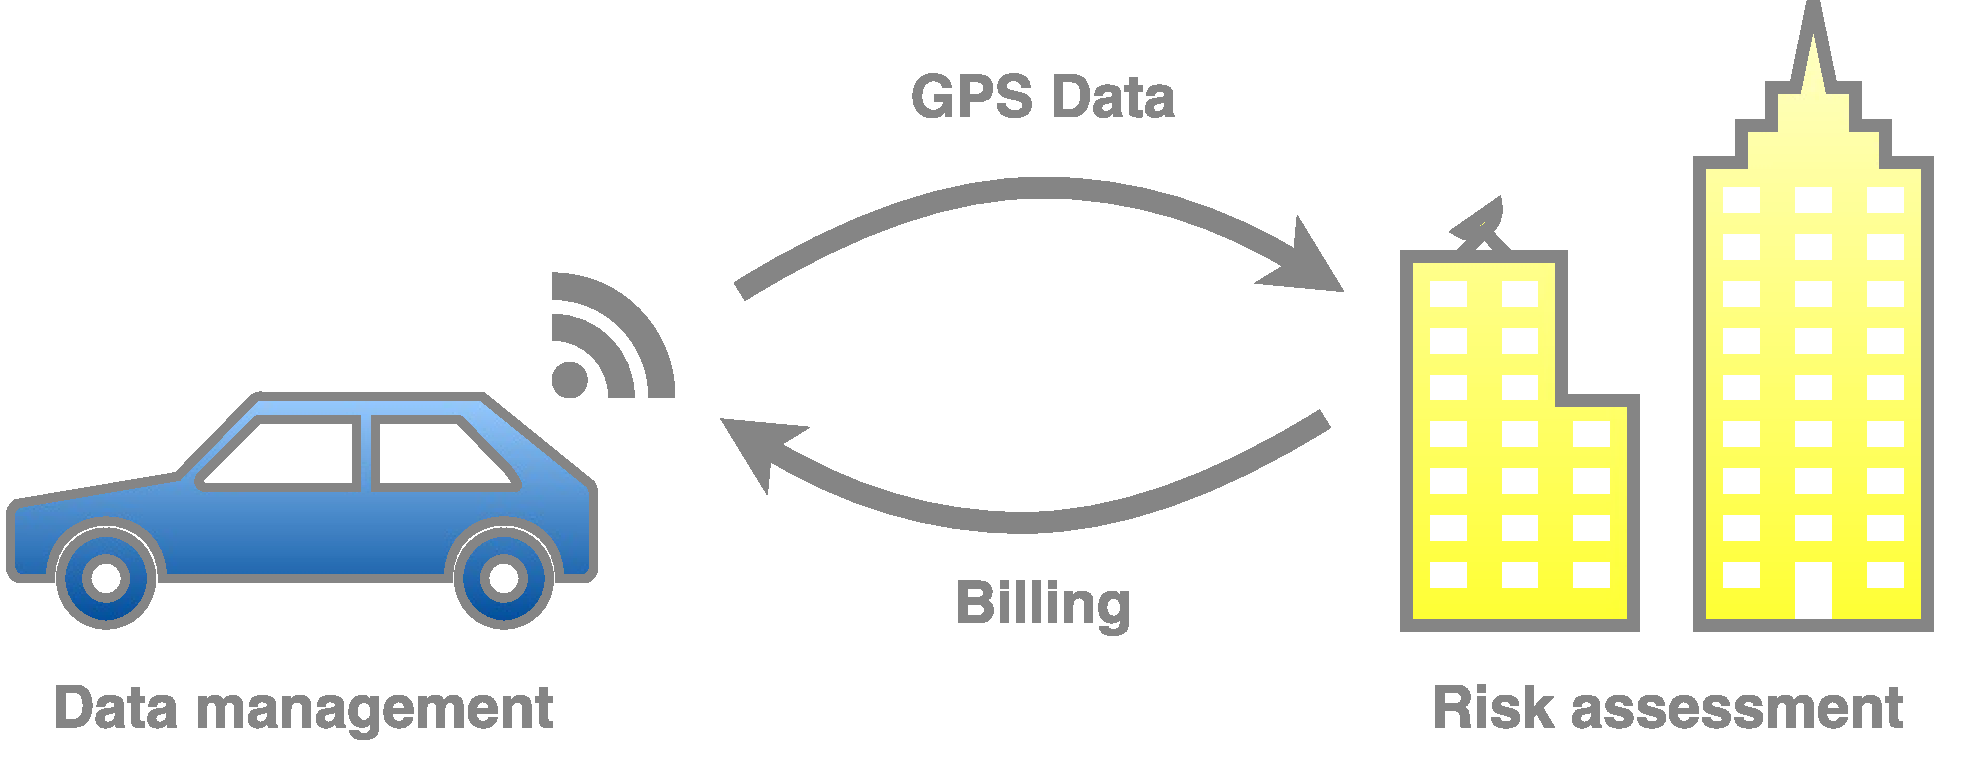
\includegraphics[width=0.9\textwidth]{Pictures/Overview}
\caption{Overview of the UBI model}
\label{fig:overview}
\end{figure*}

To make insurance more fair, it makes sense to look at individuals rather than segmented groups. If risk prediction could be calculated based on the use of individual cars, that also means the customer could receive a fair price offer. This type of insurance is known as Usage Based Insurance (UBI) or Pay-As-You-Drive(PAYD), and a few insurance companies are already offering it as experimental products. The idea behind this type of insurance can be seen in figure \ref{fig:overview}. The customer is tracked by GPS, and transmits the logged data to the insurance company. The company then bills the customer according to the received data, and is able to refine risk assessment and policies by including the newest data into their statistics.
By example, the American insurance company \texttt{Progressive} sells UBI in selected states under the name \texttt{Snapshot}\cite{snapshot}. The insurance requires the customer to have Progressive's own GPS device mounted in their cars, inserted into an OBD-II port. The device measures distance driven, number of hard braking events and more, which is transmitted to \texttt{Progressive}. The customer can then go online to see personal billing information along with a summary of the registered data.

A common factor for any UBI system is the requirement for certain hardware in the insured cars. The insurance company needs data, which the device must provide. The data is usually sent directly from the device to the insurance company, which is also the case in the before mentioned example. This model can however be a concern for the customer. The data can be inaccessible, since it is sent directly to the insurance company. The insurance company then decides which data the customer can see, and it might not be possible to verify if you are being billed correctly. Furthermore, it is not transparent which data the insurance company actually collects and stores about you and your car. In Progressive's example it can be read from their FAQ that "some devices collect location data", which may be a privacy concern, especially given that the data can not be accessed.

This paper suggest how to alleviate privacy concerns of the policyholder, while still maintaining a logical billing scheme that works for the insurance company. It provides a data warehouse to store large amounts of spatio-temporal data, with efficient and easy querying in mind. The data warehouse is logically split between privacy-sensitive customer data and less sensitive insurance company data. The solution facilitiates gamification in a way that allowes customers to compete for best driver titles on specific segments. This enables the insurance company to gather more descriptive data than normally, when their customers allow it. The authors provide suggestions on which metrics the insurance company should make use of, inspired by \citet{art:insurtelematics} and \citet{art:smartphonemonitor}. The paper provides a series of customizable metrics, which enables insurance companies to fully control what their customers are billed for. It also provides customizable score calculations on these metrics, allowing control of the base cost of delinquencies. Furthermore, experiments have been conducted to demonstrate that the proposed solution can identify different driving patterns and produce meaningful pricing points.

The main challenges in achieving these goals lies in data management, both for supporting different metrics, but also for computing costs for billing schemes following a privacy-friendly model. It is also desirable to design a model that the user can understand and relate to, in terms of what they are being billed for.